\documentclass[12pt,UTF8]{ctexart}
\usepackage{titling,setspace}
\usepackage{enumerate,enumitem}
\usepackage{amsmath,amssymb,amsfonts}
\usepackage{listings}
\usepackage{comment}
\usepackage{float}
\usepackage{graphicx}
\usepackage{multicol,multirow}
\usepackage{fancyhdr} % 页眉
\usepackage{ctex,titlesec}
\usepackage[export]{adjustbox} % 图片左对齐
\usepackage[unicode=true,%本行非常重要 支持中文目录hyperref CJKbookmarks对二级目录没用
	colorlinks,
	linkcolor=black,
	anchorcolor=black,
	citecolor=black,
	CJKbookmarks=false]{hyperref}
\usepackage{xcolor}
\usepackage{geometry}
\geometry{top=25.4mm,bottom=25.4mm,left=31.8mm,right=31.8mm}
\pagestyle{plain}%删除页眉
\CTEXsetup[format={\large\bfseries}]{section}
\renewcommand\maketitlehooka{\null\mbox{}\vfill} % 标题页
\renewcommand\maketitlehookd{\vfill\null}

\newcommand{\chuhao}{\fontsize{42.2pt}{\baselineskip}\selectfont}
\newcommand{\xiaochu}{\fontsize{36.1pt}{\baselineskip}\selectfont}
\newcommand{\yihao}{\fontsize{26.1pt}{\baselineskip}\selectfont}
\newcommand{\xiaoyi}{\fontsize{24.1pt}{\baselineskip}\selectfont}
\newcommand{\erhao}{\fontsize{22.1pt}{\baselineskip}\selectfont}
\newcommand{\xiaoer}{\fontsize{18.1pt}{\baselineskip}\selectfont}
\newcommand{\sanhao}{\fontsize{16.1pt}{\baselineskip}\selectfont}
\newcommand{\xiaosan}{\fontsize{15.1pt}{\baselineskip}\selectfont}
\newcommand{\sihao}{\fontsize{14.1pt}{\baselineskip}\selectfont}
\newcommand{\xiaosi}{\fontsize{12.1pt}{\baselineskip}\selectfont}
\newcommand{\wuhao}{\fontsize{10.5pt}{\baselineskip}\selectfont}
\newcommand{\xiaowu}{\fontsize{9.0pt}{\baselineskip}\selectfont}
\newcommand{\liuhao}{\fontsize{7.5pt}{\baselineskip}\selectfont}
\newcommand{\xiaoliu}{\fontsize{6.5pt}{\baselineskip}\selectfont}
\newcommand{\qihao}{\fontsize{5.5pt}{\baselineskip}\selectfont}
\newcommand{\bahao}{\fontsize{5.0pt}{\baselineskip}\selectfont}
\titleformat{\section}{\xiaosi\bfseries}{\chinese{section}、 }{0em}{}
\titleformat{\subsection}{\wuhao\bfseries}{\arabic{subsection}. }{0em}{}
% \titlespacing*{hcommandi}{hlefti}{hbefore-sepi}{hafter-sepi}[hright-sepi]
\titlespacing*{\section}{0pt}{3pt}{3pt}
\titlespacing*{\section}{0pt}{0pt}{0pt}

\setenumerate[1]{itemsep=0pt,partopsep=0pt,parsep=\parskip,topsep=5pt}
\setitemize[1]{itemsep=0pt,partopsep=0pt,parsep=\parskip,topsep=5pt}

\lstdefinelanguage[mips]{Assembler}{%
  % so listings can detect directives and register names
  alsoletter={.\$},
  % strings, characters, and comments
  morestring=[b]",
  morestring=[b]',
  morecomment=[l]\#,
  % instructions
  morekeywords={[1]abs,abs.d,abs.s,add,add.d,add.s,addi,addiu,addu,%
    and,andi,b,bc1f,bc1t,beq,beqz,bge,bgeu,bgez,bgezal,bgt,bgtu,%
    bgtz,ble,bleu,blez,blt,bltu,bltz,bltzal,bne,bnez,break,c.eq.d,%
    c.eq.s,c.le.d,c.le.s,c.lt.d,c.lt.s,ceil.w.d,ceil.w.s,clo,clz,%
    cvt.d.s,cvt.d.w,cvt.s.d,cvt.s.w,cvt.w.d,cvt.w.s,div,div.d,div.s,%
    divu,eret,floor.w.d,floor.w.s,j,jal,jalr,jr,l.d,l.s,la,lb,lbu,%
    ld,ldc1,lh,lhu,li,ll,lui,lw,lwc1,lwl,lwr,madd,maddu,mfc0,mfc1,%
    mfc1.d,mfhi,mflo,mov.d,mov.s,move,movf,movf.d,movf.s,movn,movn.d,%
    movn.s,movt,movt.d,movt.s,movz,movz.d,movz.s,msub,msubu,mtc0,mtc1,%
    mtc1.d,mthi,mtlo,mul,mul.d,mul.s,mulo,mulou,mult,multu,mulu,neg,%
    neg.d,neg.s,negu,nop,nor,not,or,ori,rem,remu,rol,ror,round.w.d,%
    round.w.s,s.d,s.s,sb,sc,sd,sdc1,seq,sge,sgeu,sgt,sgtu,sh,sle,%
    sleu,sll,sllv,slt,slti,sltiu,sltu,sne,sqrt.d,sqrt.s,sra,srav,srl,%
    srlv,sub,sub.d,sub.s,subi,subiu,subu,sw,swc1,swl,swr,syscall,teq,%
    teqi,tge,tgei,tgeiu,tgeu,tlt,tlti,tltiu,tltu,tne,tnei,trunc.w.d,%
    trunc.w.s,ulh,ulhu,ulw,ush,usw,xor,xori},
  % assembler directives
  morekeywords={[2].align,.ascii,.asciiz,.byte,.data,.double,.extern,%
    .float,.globl,.half,.kdata,.ktext,.set,.space,.text,.word},
  % register names
  morekeywords={[3]\$0,\$1,\$2,\$3,\$4,\$5,\$6,\$7,\$8,\$9,\$10,\$11,%
    \$12,\$13,\$14,\$15,\$16,\$17,\$18,\$19,\$20,\$21,\$22,\$23,\$24,%
    \$25,\$26,\$27,\$28,\$29,\$30,\$31,%
    \$zero,\$at,\$v0,\$v1,\$a0,\$a1,\$a2,\$a3,\$t0,\$t1,\$t2,\$t3,\$t4,
    \$t5,\$t6,\$t7,\$s0,\$s1,\$s2,\$s3,\$s4,\$s5,\$s6,\$s7,\$t8,\$t9,%
    \$k0,\$k1,\$gp,\$sp,\$fp,\$ra},
}[strings,comments,keywords]
\lstset{language=[mips]Assembler,basicstyle=\tiny,escapechar=`,showstringspaces=false}
\setlength{\droptitle}{-100pt}%减少标题与页眉距离

\title{

\includegraphics[width=0.2\linewidth,left]{../SYSU.png}~\\[1cm]
\textbf{\yihao 《计算机组成原理实验》\\\chuhao实验报告\\\quad\\\xiaoyi(实验一)}
}

\vspace{100pt}

\author{}
\date{}

\newcommand{\myuline}[1]{\begin{tabular}{c}#1\\\hline\end{tabular}}

\begin{document}

\clearpage\maketitle
\thispagestyle{empty}

\vspace{100pt}
\begin{spacing}{1.5}
\xiaoer
\begin{center}
\begin{tabular}{rc}
\makebox[6.2em][s]{\textbf{学\hspace{\fill}院\hspace{\fill}名\hspace{\fill}称}} : & 数据科学与计算机学院\\
\cline{2-2}\makebox[6.2em][s]{\textbf{专业(班级)}} : & 17级计科教务一班\\
\cline{2-2}\makebox[6.2em][s]{\textbf{学\hspace{\fill}生\hspace{\fill}姓\hspace{\fill}名}} :& 陈鸿峥\\
\cline{2-2}\makebox[6.2em][s]{\textbf{学\hspace{\fill}号}} : & 17341015\\
\cline{2-2}\makebox[6.2em][s]{\textbf{时\hspace{\fill}间}} : & 2018 年 10 月 10 日\\
\cline{2-2}
\end{tabular}
\end{center}
\end{spacing}

\newpage
\pagestyle{fancy}
\lhead{}
\rhead{\xiaowu\color{gray}{计算机组成原理实验}}
\setcounter{page}{1}
\quad\bigskip\bigskip
\rightline{\erhao\textbf{\underline{成绩:\qquad\quad}}}
\vspace{20pt}
\leftline{\erhao\textbf{\underline{实验一:MIPS汇编语言程序设计实验}}}
\vspace{-20pt}

\begin{spacing}{1.1}
\wuhao
\section{实验目的}
\begin{enumerate}
	\item 初步认识和掌握MIPS汇编语言程序设计的基本方法
	\item 熟悉PCSpim模拟器的使用
\end{enumerate}


\section{实验内容}
% 实验的具体内容与要求
\qquad从键盘输入10个无符号数或从内存中读取10个无符号字,并从大到小进行排序,排序结果在屏幕上呈现。


\section{实验器材}
\qquad电脑一台、PCSpim仿真器软件一套。


\section{实验过程与结果}
% 说明:根据需要书写相关内容,如:
% 程序流程图、设计的思想与方法、分析、实验步骤和实验结果及分析等。
\subsection{思想方法与程序流程图}
\par 由于汇编对大量数的判断和交换比较麻烦,故本程序采用复杂度较高但较容易实现的\textbf{选择排序}对这10个整数进行排序。
\par 设存储10个整数的数组为$arr$。在第$i$个循环,在$arr[j],j\in[i,10]$中选取最大的数,将其放置到$arr[i]$个位置(交换$arr[i]$与$arr[maxIndex]$,经过$9$次循环可实现对整数的排序。
程序流程如图\ref{fig:sorting}所示。
\begin{figure}[htbp]
	\centering
	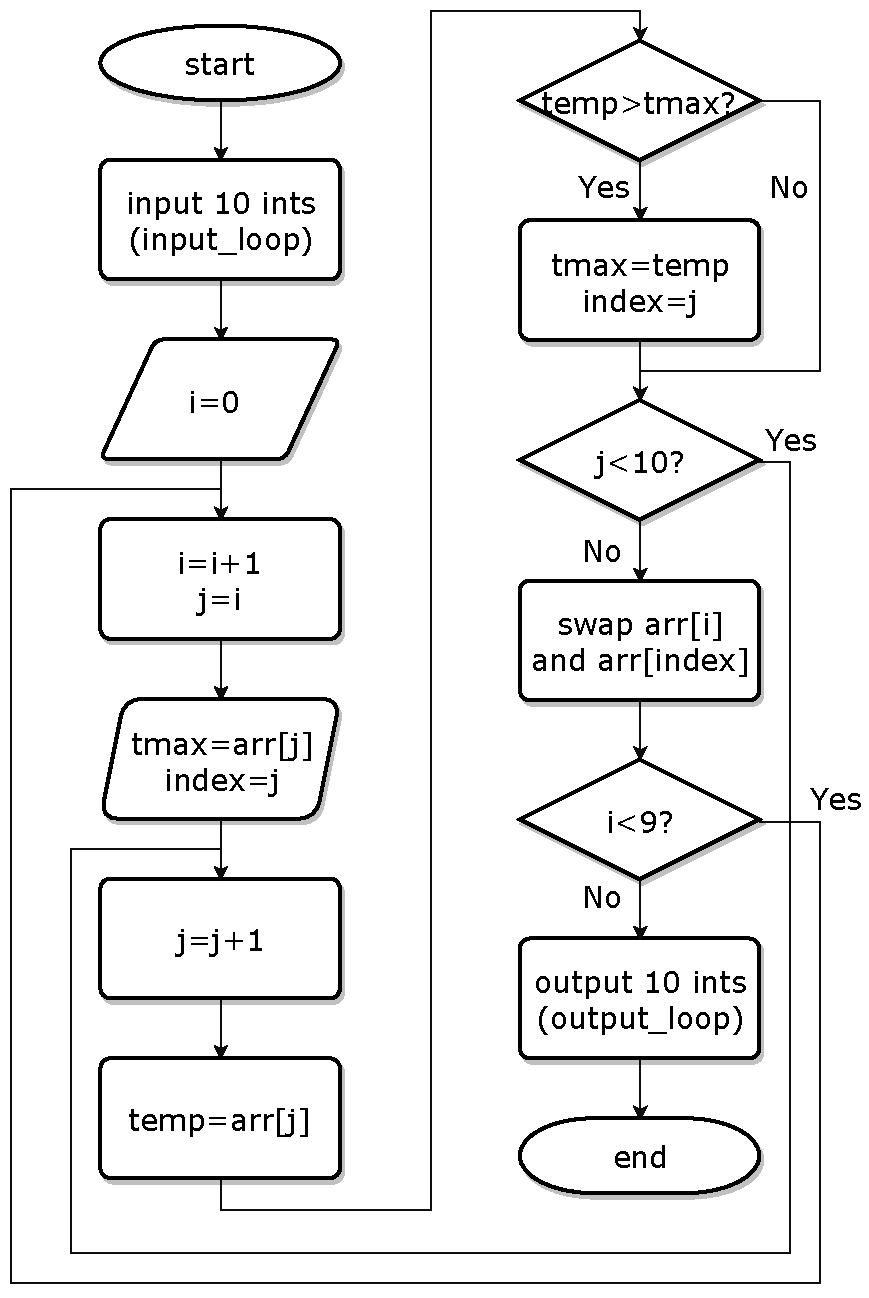
\includegraphics[width=0.6\linewidth]{fig/selection_sort.pdf}
	\caption{选择排序}
	\label{fig:sorting}
\end{figure}
\par 注意本流程图对输入输出进行了简化处理,实际上也是需要进行循环判断跳转的,详情可见第\ref{sec:program}节-程序清单。

\subsection{实验步骤}
\begin{enumerate}
	\item 随机选取10个正数输入,注意是无符号数,故不考虑负数
	\item 观察实验输出,并分析结果
	\item 重复实验3次
\end{enumerate}

\subsection{结果与分析}
\par 第一次实验数据:1 8 4 7 2 6 9 5 0 3,正常输入,结果见图\ref{fig:exp}左。
\par 第二次实验数据:52 100 1 8 2 8 99 5 6 32,考虑数之间极差较大的情况,结果见图\ref{fig:exp}中。
\par 第三次实验数据:1 2 2 2 2 3 3 3 3 3,考虑多个数都相等的情况,结果见图\ref{fig:exp}右。
\begin{figure}[htbp]
	\centering
	\begin{tabular}{ccc}
	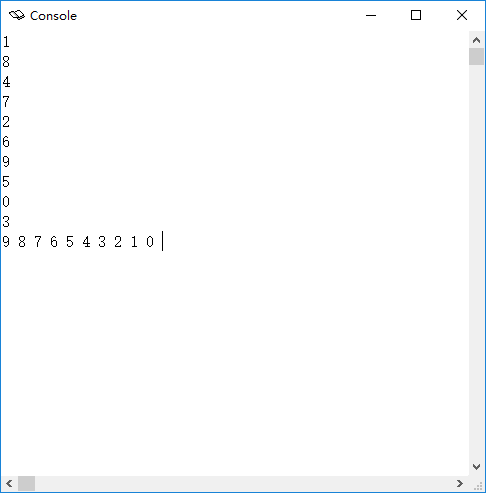
\includegraphics[width=0.33\linewidth]{fig/exp_1.PNG}&
	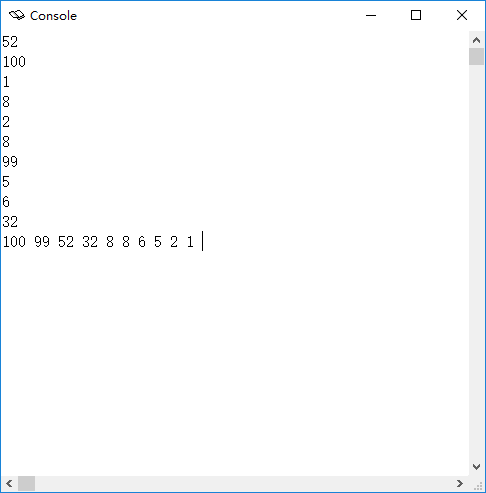
\includegraphics[width=0.33\linewidth]{fig/exp_2.PNG}&
	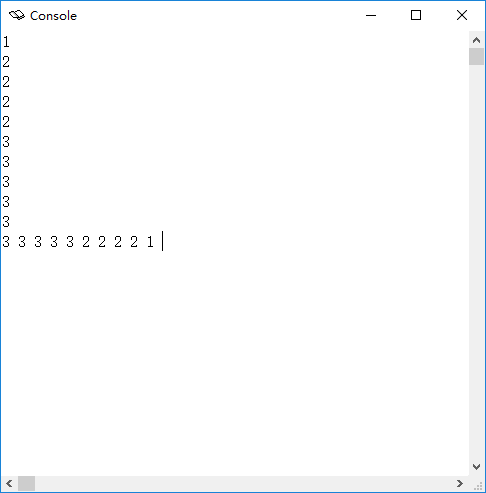
\includegraphics[width=0.33\linewidth]{fig/exp_3.PNG}
	\end{tabular}
	\caption{实验结果,由左到右分别为第一次、第二次、第三次}
	\label{fig:exp}
\end{figure}
\par 由上面实验的结果都可以发现,程序正常执行,没有报错,且正确将10个整数由大到小排序后输出到屏幕。


\section{实验心得}
% 体会和建议。(必须认真写,若过于简单,扣分!)
% (所写内容,如实验的整个过程中,所碰到的问题、所思考的问题等,以及最后如何获得解决,从中得到什么?等等,当然,还可能存在未解决的问题,或有所建议等。整个来说,就是总结一下本实验的情况,温故而知新,这个道理显而易见。)
本次实验为第一次手写汇编代码,思考很多也获益良多,总结如下。
\begin{enumerate}
	\item 首先最重要的一点是学会了MIPS的代码结构和基本语法。MIPS与高级语言C/C++相似,都有主函数入口main,通过\verb'.globl main'声明。高级语言对于常量的声明可以在任意地方,但MIPS会有专门的数据域(\verb'.data'),存放空间大小(\verb'.space')、字符串(\verb'.asciiz')等。
	\item MIPS对于数组的管理都需要自己声明空间并计算地址位置,由于int为4字节,故数组索引时每次要增加4,这个数组索引是需要与循环计数器区别开来单独计算的。
	\item MIPS比较麻烦的一点在于各个寄存器不能给其声明别名(也可能是因为我不会),导致写到后面经常会忘记某个寄存器用没用,它的作用是什么。为解决这个问题,我在主函数前特意加了几行注释说明使用到的寄存器分别用来存放什么数据,后面撰写代码时就严格执行。
	\item MIPS的循环通常是高级语言中的\verb'do...while'类型,意味着要考虑第一次进入循环执行的情况,由于数字数量$N=10>2$是确定的,故选择排序中的内层循环必然要执行,相当于把问题简化了,不用再判断循环是否执行。
	\item MIPS里的循环计数需要自己控制,通常通过判断指令\verb'slt'和跳转指令\verb'bnez'共同实现。同时要在对应地方加上loop标号,便可实现循环体内的命令不断执行。
	\item 至于写汇编代码的感受:汇编代码一定要一气呵成,需要的脑力非常大,相当于人脑作为计算机模拟,需要时刻保持清醒,对其中的逻辑要十分清楚,否则断断续续会导致效率极低,且最终出现bug调试难度大。
	\item 写汇编一定要有良好的代码结构,缩进要对齐,同时每行加上注释,原因同上。
	\item 最后,本次实验存在的问题是问题规模太小了,而且采用$\mathcal{O}(n^2)$的排序算法,但却是对MIPS汇编语言很好的探索。本来想着实现其他$\mathcal{O}(n\log n)$的排序算法,但考虑到堆排序、快速排序等的实现难度,以后可以继续探讨。
\end{enumerate}

\section{程序清单}
\label{sec:program}
\begin{lstlisting}
# Copyright 2018, SYSU
# Author: Chen Hongzheng, Major in Computer Science (17), SDCS, SYSU
# E-mail: chenhzh37@mail2.sysu.edu.cn
# Date: 2018/10/09
# This is a simple sorting (selection, inverse ordering) program for 10 numbers.

.text
.globl main

# ------------ register description -------------
# $s7=10, $s6=9              loop boundary (constant)
# $t0(out), $t1(in)          array address
# $t7(out), $t6(in)          loop counter
# $t9(out), $t8(in)          bool value used for loop termination judgement
# $s1(curr), $s2(global)     temporary value used for find the maximum
# $s0=arr[$t0], $s1=arr[$t1]
# $t2                        maximum address
# $v0                        system function call (input/output)

# ----------- main function segment -------------
main:
# -------------------- input --------------------
    addi    $s7,    $zero,    10       # loop boundary
    add     $t7,    $zero,    $zero    # counter
    la      $t0,    array              # address of the array
input_loop:
    addi    $t7,    $t7  ,    1        # $t7<-$t7+1, start from 1
    li      $v0,    5                  # load integer
    syscall
    addi    $t0,    $t0  ,    4        # calculate the address of arr[$t0], start from arr[1]
    sw      $v0,    0($t0)             # store the input number into arr[$t0]

    slt     $t9,    $t7  ,    $s7      # $t7<10 ? $t9=1 : $t9=0
    bnez    $t9,    input_loop         # $t9!=0  ? loop  : continue

# ------------------- sorting -------------------
    addi    $s7,    $zero,    10       # loop boundary
    addi    $s6,    $zero,    9        # outer loop boundary, NOTE THAT NOT 10!
    add     $t7,    $zero,    $zero    # outer_counter
    la      $t0,    array              # address of the array
outer_loop:
    addi    $t7,    $t7  ,    1        # $t7<-$t7+1, start from 1
    addi    $t0,    $t0  ,    4        # calculate the address of arr[$t0], start from arr[1]
    lw      $s0,    0($t0)             # load arr[$t0] from the memory

    add     $t6,    $t7  ,    $zero    # inner_counter initialization, $t6=$t7
    add     $t1,    $t0  ,    $zero    # initialize the address, $t1=$t0
    lw      $s2,    0($t0)             # load arr[$t0] as the initial maximum
    addi    $t2,    $t0  ,    0        # initial maximum address, $t0

    # !!! since there're 10 numbers, inner loop must be executed 
    inner_loop:
        addi $t6,    $t6,     1        # $t6<-$t6+1, start from $t7+1
        addi $t1,    $t1,     4        # calculate the address of arr[$t1], start from arr[$t0+1]
        lw   $s1,    0($t1)            # load arr[$t1] from the memory

        slt  $t8,    $s1,     $s2      # arr[$t0]<$s2, do nothing
        bnez $t8,    no_update         # update or not
        add  $s2,    $s1,     $zero    # update the maximum
        add  $t2,    $t1,     $zero    # update the maximum address

        no_update:
        slt  $t8,    $t6,     $s7      # $t6<10 ? continue : break
        bnez $t8,    inner_loop
    
    # swap two numbers, $s0 has been the temporary variable
    sw      $s2,     0($t0)            # store the maximum into arr[$t0]
    sw      $s0,     0($t2)            # store original arr[$t0] into arr[$t2]

    # loop condition
    slt     $t9,     $t7,     $s6      # $t7<9 ? continue : break
    bnez    $t9,     outer_loop

# -------------------- output -------------------
    addi    $s7,    $zero,    10       # loop boundary
    add     $t7,    $zero,    $zero    # counter
    la      $t0,    array              # address of the array
output_loop:
    addi    $t7,    $t7  ,    1        # $t7<-$t7+1, start from 1
    addi    $t0,    $t0  ,    4        # calculate the address of arr[$t0], start from arr[1]
    lw      $a0,    0($t0)             # load arr[$t0]
    li      $v0,    1                  # print integer
    syscall
    la      $a0,    nline              # prepare for output
    li      $v0,    4                  # print space
    syscall

    slt     $t9,    $t7  ,    $s7      # $t7<$s7 ? $t9=1 : $t9=0
    bnez    $t9,    output_loop        # $t9!=0  ? loop  : continue

# --------------------- exit --------------------
    li      $v0,    10                 # exit
    syscall

# ------------- data field segment --------------
.data
    array:     .space  44              # 11*4=44bytes, int for 4 bytes
    inputline: .asciiz "Please enter 10 numbers to sort: "
    nline:     .asciiz " "
\end{lstlisting}
\end{spacing}

\end{document}